% CVPR 2026 submission.
% Use with the official CVPR 2026 author kit: this project must contain the
% official cvpr.sty and ieeenat_fullname.bst (from the CVPR author kit /
% Overleaf CVPR 2026 template). This file is self-contained otherwise
% (no separate preamble.sty is needed).

\documentclass[10pt,twocolumn,letterpaper]{article}

%%%%%%%%% PAPER TYPE  - PLEASE UPDATE FOR FINAL VERSION
%\usepackage{cvpr}              % To produce the CAMERA-READY version
\usepackage[review]{cvpr}       % To produce the REVIEW version
%\usepackage[pagenumbers]{cvpr} % To force page numbers, e.g. for an arXiv version

% Standard packages (order matters: load these before hyperref).
\usepackage{graphicx}
\usepackage{amsmath}
\usepackage{amssymb}
\usepackage{amsfonts}
\usepackage{booktabs}
\usepackage{multirow}
\usepackage{array}
\usepackage{dsfont}   % provides \mathds{1} (indicator function)
\usepackage{xspace}

% It is strongly recommended to use hyperref, especially for the review version.
\usepackage[pagebackref,breaklinks,colorlinks,allcolors=cvprblue]{hyperref}

\definecolor{cvprblue}{rgb}{0.21,0.49,0.74}
\usepackage[capitalize]{cleveref}
\crefname{section}{Sec.}{Secs.}
\Crefname{section}{Section}{Sections}
\Crefname{table}{Table}{Tables}
\crefname{table}{Tab.}{Tabs.}

% Abbreviation macros (guarded: the official cvpr.sty usually defines these,
% in which case \providecommand is a harmless no-op).
\providecommand{\etal}{\textit{et al}.\@\xspace}
\providecommand{\ie}{\textit{i.e}.\@\xspace}
\providecommand{\eg}{\textit{e.g}.\@\xspace}

% Float placement: this table-dense paper needs generous limits so floats are
% placed near their references (top or bottom of page) rather than deferred.
\setcounter{topnumber}{3}
\setcounter{bottomnumber}{2}
\setcounter{totalnumber}{5}
\renewcommand{\topfraction}{0.92}
\renewcommand{\bottomfraction}{0.9}
\renewcommand{\textfraction}{0.06}
\renewcommand{\floatpagefraction}{0.75}

%%%%%%%%% PAPER ID  - PLEASE UPDATE
\def\paperID{*****} % *** Enter the Paper ID here
\def\confName{CVPR}
\def\confYear{2026}

\begin{document}

%%%%%%%%% TITLE - PLEASE UPDATE
\title{Seeing  Better but Knowing Less: Corruption-Robustness Fine-Tuning Silently Erodes
Visual Abstention in Vision-Language Models}

\author{Anonymous CVPR submission\\
Paper ID \paperID}

\maketitle

\begin{figure*}[t]
  \centering
  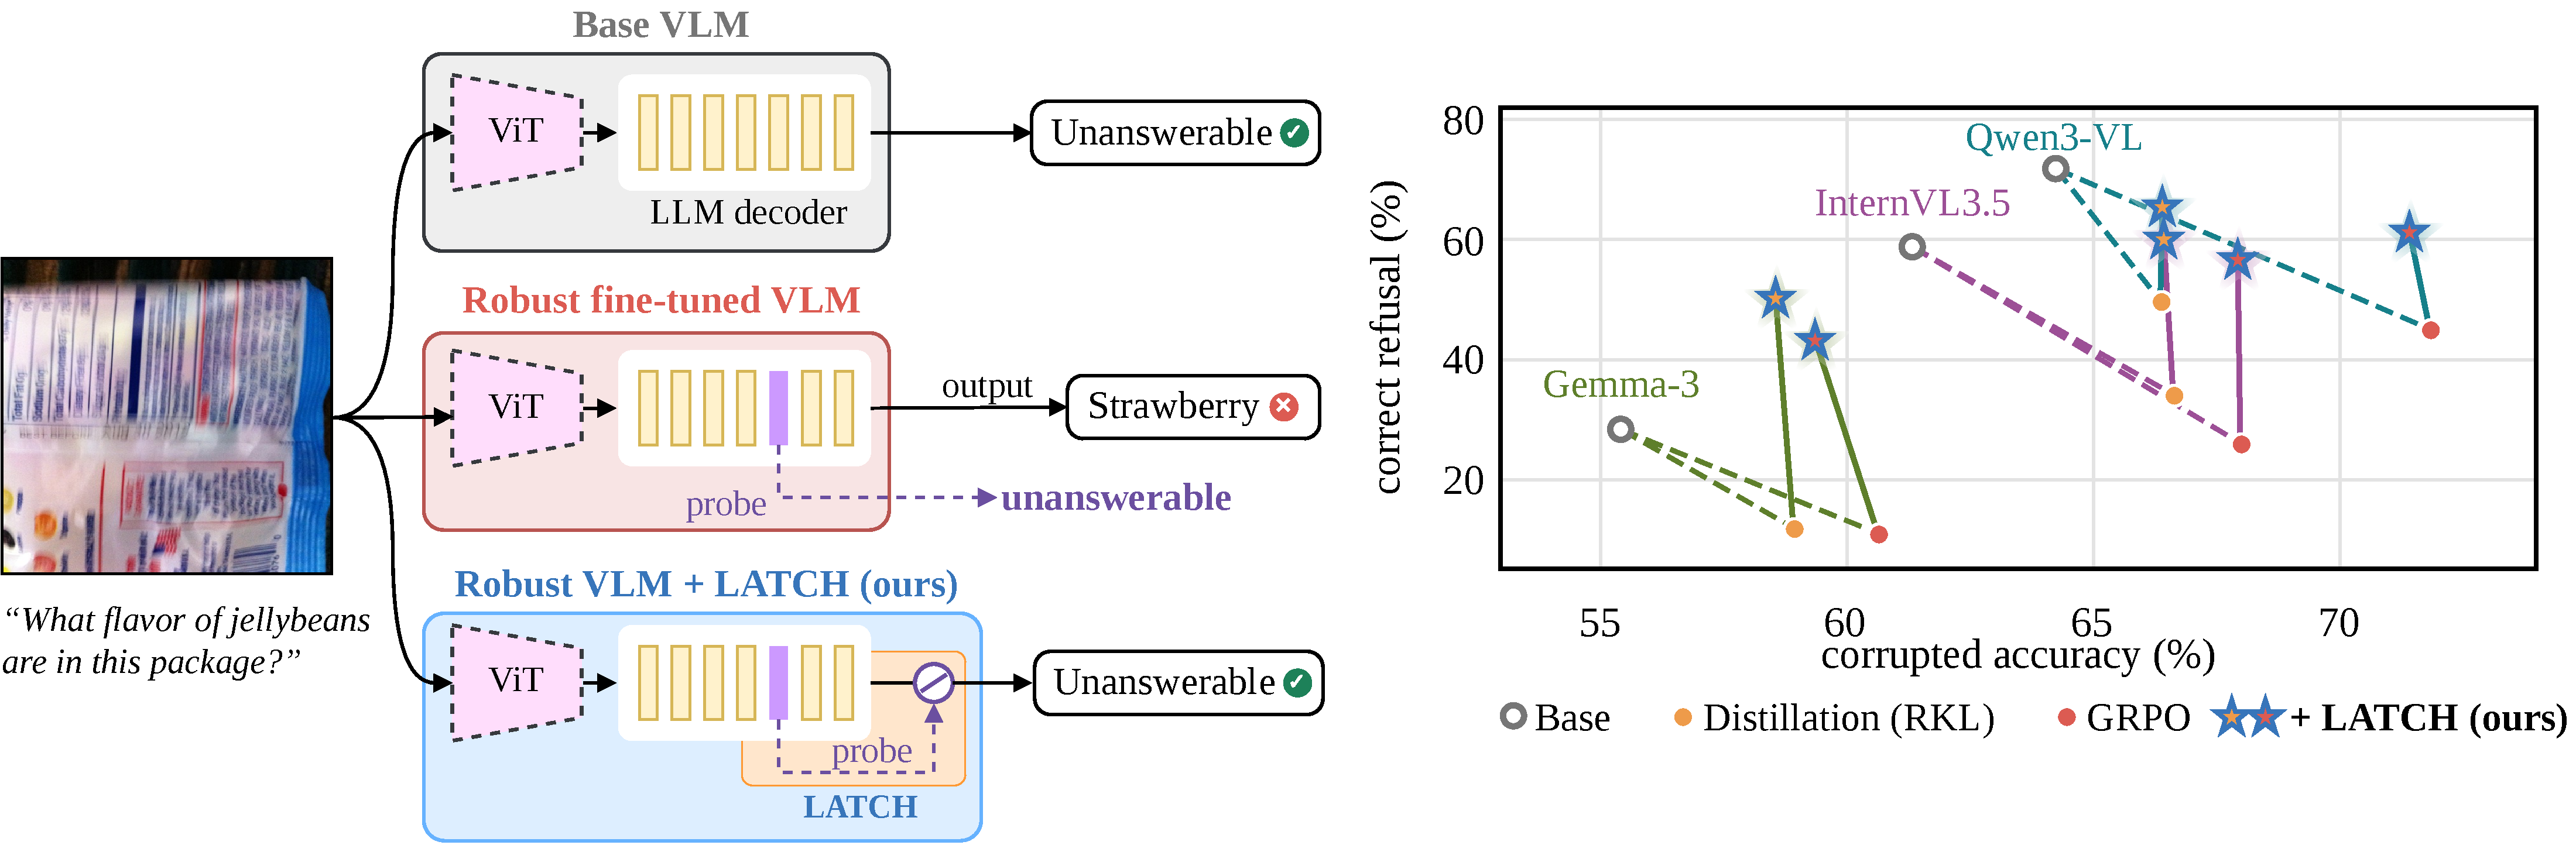
\includegraphics[width=0.9\linewidth]{figures/teaser.pdf}
  \caption{Overview of our proposed method showing how corruption robustness fine-tuning affects visual abstention across different modalities.}
  \label{fig:teaser}
\end{figure*}
%%%%%%%%% ABSTRACT
\begin{abstract}
Vision--language models (VLMs) are deployed precisely where images are hardest to
read: assistive photography for blind and low-vision users, perception through rain,
fog and motion blur, and low-quality clinical or scientific scans. In these settings
the safe response to an uninterpretable input is not a confident guess but an
admission that the image cannot support an answer. We show that the obvious way to
prepare a VLM for degraded inputs---fine-tuning it for corruption robustness---silently
removes this behavior. Using two standard adaptation recipes, on-policy reverse-KL
distillation (RKL) and Group Relative Policy Optimization (GRPO), we find that
corruption-robust training improves clean and corrupted accuracy and transfers
zero-shot to corruption types never seen in training, yet drives both models to
answer uninterpretable and image-free inputs far more often than the base model.
The regression is invisible to accuracy: the most accurate model we train is the
worst at recognizing when it cannot see. We then explain the failure. A linear probe
recovers answerability from frozen hidden states at $\text{AUROC}\approx0.93$ in every
model, so the ability is suppressed, not erased; and a reasoning-transplant test shows
the two recipes break for opposite reasons---RKL cannot reason its way to
``unanswerable,'' whereas GRPO reasons correctly but has learned an answer-level
shortcut that commits regardless. Finally we recover abstention two ways---adding
$10\%$ unanswerable examples to training, and inference-time activation steering toward
the base model---each at no cost to the corruption gains, with the training objective
deciding which works better. The results argue that corruption robustness and
calibrated abstention must be measured, and optimized, together.
\end{abstract}

%%%%%%%%% BODY TEXT
\section{Introduction}
\label{sec:intro}

Vision--language models are most useful in exactly the conditions that most degrade
an image. Assistive applications answer questions about photographs taken by blind
and low-vision users, who cannot verify whether a shot is focused, framed, or
lit~\cite{gurari2018vizwiz}; perception systems in vehicles must see through rain, fog,
glare and motion; and scientific and clinical tools routinely operate on noisy scans.
What unites these settings is a single property: a confident wrong answer is the most
damaging possible output, because whoever acts on it receives no signal that it is
wrong. When an input is genuinely uninterpretable, the correct behavior is
\emph{abstention}---stating that the image does not support an answer.

VLMs are notoriously bad at this. Across a growing body of
benchmarks~\cite{miyai2024upd,zhu2025mohobench,saadat2025visiontrap,
madhusudhan2026knowing}, state-of-the-art models answer unanswerable visual questions
rather than withhold, and recent work shows the deficit is not one of perception but of
expression: a model's hidden states often encode that an input is unanswerable while its
output commits to an answer anyway. This \emph{representation--output gap} has been
documented from several directions---linear probes that decode answerability which the
response ignores~\cite{he2026knowing,pramono2026trapsbench}, calibration
metrics~\cite{chandu2025certainly}, and the broader finding that language models
internally ``know what they know'' more than they say~\cite{kadavath2022know,
burns2023discovering}. What this literature has in common is that it characterizes the
gap in \emph{off-the-shelf} models. It leaves open a question that matters the moment one
tries to deploy a VLM in degraded conditions: what does \emph{training} the model for
those conditions do to the gap?

This is the question we study, and the answer is unwelcome. The natural way to make a
VLM robust to degraded inputs is to fine-tune it on corrupted images, and two paradigms
dominate practice. Knowledge distillation trains a student that sees a degraded image to
imitate a larger teacher that sees the clean one; it is inexpensive, needs no
ground-truth labels, and uses only teacher forward passes. Reinforcement learning with
verifiable rewards, here Group Relative Policy Optimization
(GRPO)~\cite{shao2024deepseekmath}, rewards the model when its answer matches the gold
answer. Both reliably raise accuracy on corrupted inputs---and both, we find, do
something their accuracy never reveals: they teach the model to stop abstaining. The gap
that prior work measured in static models is not fixed; a routine, well-motivated
training intervention actively widens it. This is an instance of a pattern now
familiar on the language side, where fine-tuning for one objective silently erodes a
capability it never touched~\cite{qi2024finetuning,luo2023empirical}; we give the first
account of it for visual abstention, and trace it to the training objective.

We establish this on Qwen3-VL-4B-Instruct~\cite{qwen3vl2025}, fine-tuned with on-policy
reverse-KL distillation (RKL)~\cite{gu2024minillm} and with GRPO on 30k GQA
questions~\cite{hudson2019gqa} corrupted by a 16-style engine, and evaluated on
corrupted TextVQA~\cite{singh2019textvqa}, GQA~\cite{hudson2019gqa} and
VQAv2~\cite{goyal2017vqav2} following the corruption protocol of
Usama~\etal~\cite{usama2025analysing}, together with VizWiz~\cite{gurari2018vizwiz}: real
blind-user photographs, a third of whose questions are genuinely unanswerable. The
pattern we uncover is not a quirk of one recipe but a coupling between two objectives
that the field optimizes and reports in isolation. We make four contributions.

\begin{itemize}
\item \textbf{A silent abstention regression.} Corruption-robust fine-tuning raises
clean and corrupted accuracy---with gains that transfer zero-shot to unseen
corruptions (\cref{sec:robustness})---yet answers unanswerable VizWiz questions and
image-free inputs far more often than the base model (\cref{sec:regression}). GRPO,
the most accurate model, is the worst abstainer, and no accuracy metric exposes this.

\item \textbf{The ability is suppressed, not erased (RQ1).} A linear probe decodes
answerability from frozen hidden states at $\text{AUROC}\approx0.93$ in all three models
and still flags most of the inputs they wrongly answer; the failure is behavioral, not
representational (\cref{sec:rq1}).

\item \textbf{Two opposite failure mechanisms (RQ2).} A reasoning-transplant test shows
RKL fails on the reasoning side (given a ``can't-tell'' chain it abstains $98.4\%$ of
the time, so unaided it never reaches that chain), while GRPO fails on the answer side
(given the same chain it still answers $91.8\%$ of the time, a reward-induced shortcut)
(\cref{sec:rq2}).

\item \textbf{Two mechanism-matched remedies (RQ3).} A $10\%$ unanswerable data mix and
inference-time activation steering each restore abstention without surrendering the
corruption gains, and the objective decides which is better---entropy-gated steering
for RKL, the missing data signal for GRPO (\cref{sec:rq3}).
\end{itemize}

The lesson is methodological: corruption robustness and calibrated abstention are
coupled, standard accuracy benchmarks hide the coupling, and the right fix depends on
how the model was trained. We therefore report an explicit abstention axis beside
accuracy throughout.

\section{Related Work}
\label{sec:related}

\paragraph{VLMs and visual question answering.}
Instruction-tuned VLMs built on strong language backbones are now the default interface
for image understanding~\cite{qwen3vl2025}. They are measured on VQA benchmarks
targeting compositional reasoning (GQA~\cite{hudson2019gqa}), language-prior control
(VQAv2~\cite{goyal2017vqav2}), and scene-text reading (TextVQA~\cite{singh2019textvqa}).
VizWiz~\cite{gurari2018vizwiz} is unique for our purpose: its images are taken by blind
users, are frequently unreadable, and a large share of its questions cannot be answered,
making it the natural testbed for abstention under real-world degradation.

\paragraph{Corruption robustness for VLMs.}
ImageNet-C~\cite{hendrycks2019imagenetc} established common corruptions---noise, blur,
weather and digital artifacts at graded severity---as the standard average-case
robustness benchmark, distinct from worst-case adversarial robustness. The behavior of
VLMs under these corruptions has only recently been quantified:
Usama~\etal~\cite{usama2025analysing} apply the $19$ ImageNet-C corruptions at five
severities to TextVQA and GQA, finding that VQA accuracy degrades substantially and
unevenly across corruption families. We adopt their corrupted-VQA evaluation protocol but
depart from it in two ways that make our robustness claims stronger: we \emph{train} for
robustness rather than only measuring it, and we train with a different, disjoint
corruption engine, so that most evaluation corruptions are unseen and the measured gains
reflect generalization rather than memorized pixel statistics.

\paragraph{Distillation and RL for adaptation, and their side effects.}
Knowledge distillation~\cite{hinton2015distilling} transfers a teacher's behavior to a
student; for generative models, MiniLLM~\cite{gu2024minillm} shows that reverse KL is
preferable to forward KL because it is mode-seeking and avoids placing mass on regions
the teacher never visits. Our distillation is on-policy reverse-KL with a clean-image
teacher and a corrupted-image student. On the RL side, GRPO~\cite{shao2024deepseekmath}
replaces PPO's value network~\cite{schulman2017ppo} with group-relative advantages from
sampled rollouts, and is a common recipe for verifiable-reward fine-tuning;
LoRA~\cite{hu2022lora} is a standard efficient variant of both. Neither recipe is
side-effect free. Fine-tuning is now known to degrade capabilities it never targets:
benign fine-tuning erodes safety alignment~\cite{qi2024finetuning}, and continual
adaptation induces catastrophic forgetting~\cite{luo2023empirical}. Reward-based training
additionally invites shortcut behavior, where the policy satisfies the reward through a
spurious regularity rather than the intended competence. Our GRPO result is a clean,
causally demonstrated instance of such a shortcut---\emph{always answer}---surfacing
specifically in the abstention setting, where the reward is defined only over answerable
inputs.

\paragraph{Visual abstention and the representation--output gap.}
Knowing when not to answer is central to reliability~\cite{geifman2017selective}, and the
problem is acute for VLMs, which readily produce confident answers to unanswerable or
image-free prompts. In language, SQuAD~2.0~\cite{rajpurkar2018squad2} and
AbstentionBench~\cite{kirichenko2025abstentionbench} formalize unanswerable questions. On
the multimodal side a cluster of benchmarks now measures the failure directly: UPD
dissects it into absent-answer, incompatible-answer-set and incompatible-question
settings~\cite{miyai2024upd}; MoHoBench frames it as honesty and reports that most of $28$
models tested fail to refuse when they should~\cite{zhu2025mohobench};
VisionTrap~\cite{saadat2025visiontrap} and MM-AQA~\cite{madhusudhan2026knowing} construct
unanswerable instances from answerable ones and reach the same verdict, with MM-AQA
arguing that the bottleneck is miscalibration and that abstention-aware \emph{training},
not better prompting, is what is required. A complementary line adds the ability at low
cost: selective-prediction methods estimate answer reliability from black-box
consistency~\cite{khan2024consistency} or temper over-abstention~\cite{srinivasan2024recoverr},
and CLIP-UP attaches a light unanswerability head without touching the backbone
weights~\cite{vardi2025clipup}.

Most directly related to us are two concurrent works that locate the failure inside the
model. TRAPSBench~\cite{pramono2026trapsbench} studies physical-reasoning videos and
reports a \emph{representation--output gap}: across $16$ VLMs spontaneous restraint is
poor (best penalized calibration score $0.292$), yet linear probes decode answerability
from hidden states at up to $0.91$ AUROC and a single-layer steering direction causally
induces or suppresses abstention; tellingly, textual impossibility is detected about
$4\times$ more readily than missing visual evidence. He~\etal~\cite{he2026knowing} reach
the same diagnosis on static images---probe-decodable answerability that final responses
ignore, with spontaneous abstention recall near $11$--$16\%$---and close the gap with a
representation-to-action alignment step. CertainlyUncertain~\cite{chandu2025certainly}
similarly pairs answerable and unanswerable inputs to measure calibrated awareness.

All of this work characterizes---or repairs---the gap in a \emph{fixed} model. Our
contribution is orthogonal and, we argue, more actionable. We show that the gap is not a
static property but a \emph{moving target}: a routine, well-motivated training
intervention---fine-tuning for corruption robustness---actively widens it, in a direction
that standard accuracy benchmarks cannot see. We further show the widening is
mechanistic: it arises through two objective-specific failures (reasoning-side for
distillation, answer-side for GRPO), and can therefore be diagnosed, attributed to the
objective, and reversed without surrendering the robustness the training was meant to buy.
Our probe and steering results independently reproduce the representation--output gap in a
new regime---synthetic corruptions and real blind-user photographs rather than physics
videos---and extend it with a causal account of \emph{why training makes it worse}, a
dynamic that benchmark-only studies cannot observe.

\paragraph{Activation steering.}
Activation- and representation-engineering methods edit internal activations at inference
time to modulate a target behavior. Contrastive Activation Addition
(CAA)~\cite{rimsky2024caa} forms a steering vector from the mean difference of
residual-stream activations over positive/negative pairs and adds it during generation,
on top of fine-tuning rather than undoing it~\cite{turner2023actadd,li2023iti}; refusal
and other high-level behaviors are often mediated by a single such
direction~\cite{arditi2024refusal}. We build contrastive vectors from base-vs-trained
response pairs to push a fine-tuned model back toward the base model's abstention, and add
an entropy-gated variant matched to distillation's reasoning-side failure.

\section{Method}
\label{sec:method}

\subsection{Problem statement}
\label{sec:problem}

We consider a vision--language model $\pi$ that, given an image $x$ and a question $q$,
generates a free-form response $y = \pi(x, q)$. At deployment the image may be clean or
corrupted, $x \in \{x_{\mathrm{clean}}, \tilde{x}\}$, and the question may or may not be
answerable from it. Writing $a^\star$ for the gold answer when one exists and $\varnothing$
for ``unanswerable,'' a reliable model must satisfy two objectives at once:
\begin{enumerate}
\item \textbf{Accuracy}: return $a^\star$ when the image supports an answer, including when
the image is corrupted ($x = \tilde{x}$).
\item \textbf{Abstention}: return $\varnothing$ when it does not, whether because the image
is uninterpretable or because the evidence the question asks for is absent.
\end{enumerate}
Corruption-robust fine-tuning targets only the first objective: it trains $\pi$ so that
accuracy on corrupted inputs $\tilde{x}$ approaches accuracy on clean inputs
$x_{\mathrm{clean}}$. The second objective never enters its loss. Fine tuning on the corrupted data and trying to make the model more robust is taking away its ability to abstain or refuse to answer when the answer is not there. Our main goal is to see whether we can recover the abstention of the base model in the fine tuned model on the corrupted data. In the experiments, we will try to go into the details about why robust fine tuned models are failing to abstain in answering unanswerable questions.
\subsection{Corruption-robust fine-tuning}
\label{sec:method-ft}

We adapt a VLM to corrupted inputs with the two recipes that dominate practice. Both see a
corrupted image in place of its clean counterpart and differ only in their supervision
signal.

\paragraph{On policy distillation.}
A well known way of optimizing a model is knowledge distillation \citep{hinton2015distillingknowledgeneuralnetwork} where the model is told to follow the distribution of a more capable or differently conditioned teacher instead of using hard labels. The normal way of this fine tuning paradigm is off policy distillation where a student imitates a more capable teacher. But the problem with this is that in this paradigm of fine tuning the student blindly follows the teacher's sampled ground truth or sequence. This makes the model vulnerable to exposure bias and the student model is not corrected on the states that it reaches in reality.

The solution to this problem is on policy distillation \citep{agarwal2024onpolicydistillationlanguagemodels} where the student model is told to generate the trajectories and the teacher model corrects the states that the student produces. At each step, the student samples a rollout and the teacher provides a per token over that rollout. Reverse KL divergence is used for the loss calculation in this case where the student concentrates more on the teacher's dominant modes (Mode seeking). As a result, the student is pulled towards the teacher exactly at the states that it visits. Because the supervision is defined on the student's own distribution and there is no blind imitating, the student learns teacher's behavious where it matters the most. 


In our setting, let $\tilde{x}$ be a corrupted image, $x$ its clean counterpart, $c$ the prompt and $y$
a response. The student $q_\theta$ sees $\tilde{x}$ and is distilled toward a frozen
teacher $p_\phi$, which sees the clean image $x$. We minimize the token-level reverse
KL on-policy, sampling $G{=}2$ rollouts $y \sim q_\theta(\cdot \mid \tilde{x}, c)$ per
prompt:
\begin{equation}
\mathcal{L}_{\mathrm{RKL}}(\theta) =
\mathbb{E}_{x,\tilde{x},c,\,y\sim q_\theta}
\left[\sum_t \mathrm{KL}\!\left(q^{(t)}_\theta \,\big\|\, p^{(t)}_\phi\right)\right],
\label{eq:rkl}
\end{equation}
with $q^{(t)}_\theta = q_\theta(\cdot \mid y_{<t}, \tilde{x}, c)$ and
$p^{(t)}_\phi = p_\phi(\cdot \mid y_{<t}, x, c)$. Reverse KL is mode-seeking which in simple words mean the student
concentrates on the teacher's dominant modes~\cite{gu2024minillm}. Distillation needs no
gold answers and only teacher forward passes.

\paragraph{Group Relative Policy Optimization (GRPO).}
GRPO \citep{shao2024deepseekmathpushinglimitsmathematical} is quite similiar to the on policy distillation where the model is optimized on it's own rollouts. But instead of having a teacher teaching the model, the model is optimized using ground truths. This is a very popular way of fine tuning models in the category of reinforcement learning using veritable rewards(RLVR). For each prompt it draws a group of $G$ rollouts from the current policy and scores each against the verifiable reward. The advantage of a rollout is simply its reward standardized within the group. So the group itself supplies the baseline. This is cheaper and, for tasks with a checkable answer, well-matched to the signal available: the reward need only decide whether a sampled answer is correct.



In our setting,GRPO sees only the corrupted image. For each question it samples
$\{o_i\}_{i=1}^{G} \sim \pi_{\theta_{\mathrm{old}}}(\cdot \mid \tilde{x}, c)$ with $G{=}8$
and assigns an exact-match reward $r_i = \mathds{1}[\,\mathrm{answer}(o_i) = a^\star\,]$
against the GQA gold answer $a^\star$. Advantages are group-normalized and the policy is
updated by the clipped surrogate with a KL anchor:
\begin{equation}
\hat{A}_i = \frac{r_i - \mathrm{mean}(r)}{\mathrm{std}(r) + \varepsilon},
\label{eq:adv}
\end{equation}
\begin{equation}
\begin{aligned}
\mathcal{J}_{\mathrm{GRPO}}(\theta) = \mathbb{E}\Big[
&\frac{1}{G}\sum_{i=1}^{G}\frac{1}{|o_i|}\sum_t
\min\!\big(\rho_{i,t}\hat{A}_i,\, \bar\rho_{i,t}\hat{A}_i\big) \\
&- \beta\,\mathrm{KL}(\pi_\theta \| \pi_{\mathrm{ref}})\Big],
\end{aligned}
\label{eq:grpo}
\end{equation}
where $\rho_{i,t} = \pi_\theta(o_{i,t} \mid \tilde{x}, c, o_{i,<t}) /
\pi_{\theta_{\mathrm{old}}}(o_{i,t} \mid \tilde{x}, c, o_{i,<t})$ and
$\bar\rho_{i,t} = \mathrm{clip}(\rho_{i,t}, 1{-}\varepsilon, 1{+}\varepsilon)$. Because
the reward exists only for answerable GQA questions, nothing in \cref{eq:grpo} ever
rewards abstaining which we try to work on in the later sections.

\subsection{Recovering abstention without losing robustness}
\label{sec:method-probes}
From the results of the fine tuned models in \cref{tab:accuracy}, it is evident that the fine tuned models are doing better than the base model in case of both the clean image and corrupted image accuracy. But it is also loses its ability of not answering when the answer is not there. In this section, we discuss how can recover the abstention capability of the fine tuned model without trading the robustness gains. In our experiments, we use three ways to recover the abstention capabilities of the model which are discussed below.
% \paragraph{Answerability probe (RQ1).}
% For each VizWiz item we take the last-prompt-token hidden state $h^{(\ell)}$ at every
% layer $\ell$, before any generation. A logistic-regression probe
% $\hat{y} = \sigma(w_\ell^\top h^{(\ell)} + b_\ell)$ is trained on the VizWiz training
% split to predict answerable vs.\ unanswerable and tested on validation; a shuffled-label
% probe is the control. If a model answers inputs its own hidden states mark unanswerable,
% the failure is behavioral rather than representational.

% \paragraph{Reasoning transplant (RQ2).}
% We take unanswerable questions the trained model answered but the base model refused
% (its chain ends in ``can't tell''), prepend that base chain to the trained model, and
% measure whether it now abstains. This isolates whether a model's failure is in
% \emph{producing} the right reasoning or in \emph{acting} on it.

\paragraph{Unanswerable data augmentation}

The first remedy asks whether abstention was lost simply because the training signal never
contained it. We add a small set of ``destroyed'' examples to the training data. By destroyed examples, we mean images corrupted past the
point of recognition and labeled unanswerable (\cref{sec:setup}). This makes abstaining now a rewarded behavior, and we retrain the model from scratch under the same budget.
A single data fraction of $10\%$ tests whether the capability returns.


\paragraph{Probe switch}

 The model's internal state can still recognize the data which are not answerable which is verified and talked about in more details in \cref{sec:rq1}.We fit a linear logistic-regression probe on the residual stream at the last prompt token, the position just before the response begins, at a late decoder layer, where answerability is most cleanly decodable. The probe is trained on a held-out pool of answerable and unanswerable calibration questions disjoint from every evaluation set, and each model receives its own probe fitted to its own activations. We try to use this linear layer to recover abstention by using it as a inference time gate. Whenever the linear probe says unanswerable, we bypass the entire model's answer and just refrain from answer. Likewise, whenever the linear probe says answerable, we let the model finish its answer. 

\paragraph{Activation steering.}
Because fine-tuning suppresses abstention while leaving it decodable \cref{sec:rq1}, a third remedy restores the behavior at inference time, without retraining, by nudging the model back toward the base model’s representation of unanswerability. We add a fixed steering vector to the residual stream on generated tokens only. We steer at a layer upstream of where answerability is most decodable: answerability is already well-formed there, yet the push still lands before the tokens that commit to an answer. The vector is contrastive — the mean difference between base-model and trained-model hidden states on inputs where fine-tuning broke abstention — so it isolates the direction along which the base model’s “this input does not support an answer” representation differs from the trained model’s over-confident one. We build two such vectors, one for uninterpretable images and one for missing images. For distillation, whose failure is reasoning-side rather than answer-side (§4.2), we add an entropy-gated variant that applies the push only at high-entropy (uncertain) tokens, correcting the model’s confused steps without disturbing fluent ones. The weights are never modified, and all calibration data come from training splits with no evaluation overlap.
% \subsection{Intervention 2: activation steering}
% \label{sec:method-steer}

% The second remedy edits the model's activations at inference time, leaving the weights
% untouched. We push a fine-tuned model back toward the base model's abstention behavior
% by adding a fixed steering vector $v_{18}$ to the residual stream at layer $18$ of the
% model's $36$ layers, on generated tokens only:
% \begin{equation}
% h^{(18)}_t \leftarrow h^{(18)}_t + \lambda\, v_{18}.
% \label{eq:steer}
% \end{equation}
% All calibration data used to build the vectors come from training splits of VizWiz, GQA,
% VQAv2 and TextVQA, so there is no overlap with any evaluation set. We construct two
% complementary vectors---one for uninterpretable images and one for missing images---and,
% for distillation, an entropy-gated variant.

% \paragraph{Image-contrast steering.}
% This vector targets the case where an image is present but uninterpretable. From
% VizWiz-train photographs labelled unanswerable, we keep a question when the base model's
% answer says ``unanswerable'' and the trained model's answer does not---\ie exactly the
% questions on which fine-tuning broke abstention. For each such question we feed the same
% input (image, question, and the trained model's own response) through both models and
% take the difference of their hidden states at the positions that predict the response,
% averaged over response tokens:
% \begin{equation}
% v^{\mathrm{con}}_\ell = \operatorname*{mean}_{\text{resp.\ tokens}}
% \left[\, h^{\mathrm{base}}_\ell(x) - h^{\mathrm{trained}}_\ell(x)\,\right],
% \label{eq:vcon}
% \end{equation}
% where the shared input is $x = \text{image}+q+\text{trained response}$. This is a
% one-text, two-model contrast: the base model's response is used only to select the
% question, not fed into the vector. The difference isolates the direction in activation
% space along which the base model's ``this image does not support an answer''
% representation differs from the trained model's over-confident one. We collected $243$
% qualifying questions ($36{,}907$ response tokens) for RKL and $336$ ($27{,}386$ tokens)
% for GRPO (\cref{tab:steercalib}).

% \paragraph{No-image steering.}
% This vector targets the complementary case where no image is present at all. From
% calibration questions asked without their image, we keep a question when the base model
% refuses (a refusal word in its answer) and the trained model answers anyway, sampling
% $150$ such pairs per dataset (seed $1$). Both the base refusal and the trained answer
% are then fed through the trained model, and the vector is the mean difference between the
% two, averaged over response tokens:
% \begin{equation}
% \begin{aligned}
% v^{\mathrm{noimg}}_\ell = \operatorname*{mean}_{\text{pairs}}
% \big[\, &\bar{h}_\ell(q{+}\text{base refusal}) \\[-2pt]
% &- \bar{h}_\ell(q{+}\text{trained answer})\,\big],
% \end{aligned}
% \label{eq:vnoimg}
% \end{equation}
% where $\bar{h}_\ell$ averages layer-$\ell$ states over response tokens. This is a
% two-text, one-model contrast. Of the VizWiz-train pool only $184$ pairs qualified for
% GRPO (versus $1{,}365$ for RKL), because GRPO already refuses most no-image VizWiz
% questions---consistent with the later finding (\cref{sec:rq1}) that GRPO keeps its sense
% that the image is missing while RKL loses much of it.

% \begin{table}[tb]
% \centering
% \small
% \caption{Steering-vector calibration counts. Image-contrast: selected questions and
% response tokens. No-image: used / qualifying pairs per dataset.}
% \label{tab:steercalib}
% \begin{tabular}{@{}lcc@{}}
% \toprule
% \multicolumn{3}{c}{\textit{Image-contrast vector}} \\
% \midrule
% Model & \#Questions & \#Response tokens \\
% \midrule
% Full-FT RKL  & 243 & 36{,}907 \\
% Full-FT GRPO & 336 & 27{,}386 \\
% \bottomrule
% \end{tabular}

% \vspace{0.6em}

% \begin{tabular}{@{}lcccc@{}}
% \toprule
% \multicolumn{5}{c}{\textit{No-image vector (used / qualifying)}} \\
% \midrule
% Model & VizWiz & GQA & VQAv2 & TextVQA \\
% \midrule
% Full-FT RKL  & 150/1365 & 150/398 & 150/459 & 150/407 \\
% Full-FT GRPO & 150/184  & 150/400 & 150/460 & 150/398 \\
% \bottomrule
% \end{tabular}
% \end{table}

% \paragraph{Magnitude and placement.}
% At evaluation we add $\lambda v_{18}$ to the layer-$18$ residual stream on generated
% tokens (\cref{eq:steer}), with $\lambda{=}8$ for the image-contrast vector and
% $\lambda{=}1$ for the no-image vector, each rescaled so that the applied push matches the
% norm of a reference LoRA-RKL vector. Layer $18$ (the middle of the $36$-layer stack) is
% where the answerability representation is both well-formed and still upstream of the
% tokens that commit to an answer, matching the best-probe layers ($23$--$24$) found in
% RQ1 while leaving room for the steered representation to propagate.

% \paragraph{Entropy-gated steering, and why it is used for RKL.}
% Always-on steering perturbs every generated token, including the many tokens on which
% the model is already confident and correct. For GRPO, whose failure is a uniform
% answer-level shortcut, this is acceptable---the push is needed everywhere. For RKL,
% however, the failure is not a uniform bias but confusion during reasoning: the distilled
% model produces long, unsure chains that drift into an answer (\cref{sec:rq2}). Steering
% such a model on every token would needlessly disturb the fluent, correct parts of its
% generation and cost accuracy. We therefore gate the intervention on the model's own
% uncertainty, applying the vector at a token only when the predictive entropy of the
% next-token distribution exceeds a threshold $\tau$:
% \begin{equation}
% \text{steer at } t \iff H_t = -\sum_v p_\theta(v)\log p_\theta(v) > \tau.
% \label{eq:entropy}
% \end{equation}
% High entropy marks exactly the moments where RKL is unsure and liable to talk itself into
% an answer, which is where a nudge toward abstention should act; low-entropy tokens, where
% the model is effectively committed to a single continuation, are left untouched. We set
% $\tau = 0.5$ nats. This choice is both principled and tuned. Principled: $0.5$ nats sits
% well below $\ln 2 \approx 0.69$ (the entropy of an even two-way split) but well above the
% near-zero entropy of a confidently predicted token, so the gate fires on genuine branch
% points---where the model is weighing ``answer'' against ``abstain''---and stays silent on
% routine, committed tokens. Tuned: on calibration data $\tau = 0.5$ recovered the most
% abstention while leaving clean and corrupted accuracy essentially unchanged; lower
% thresholds approach always-on steering and begin to cost accuracy, while higher
% thresholds fire too rarely to recover abstention. Gating thus helps RKL specifically
% because its failure is reasoning-side: restricting the push to high-entropy tokens
% targets the confused steps without disturbing the rest. GRPO, whose failure is not local
% confusion, does not benefit from gating, and its no-image vector is applied directly.

\section{Experiment \& Results}
\label{sec:results}

\subsection{Experimental setup}
\label{sec:setup}

\paragraph{Backbones. \& hardwares}
We study three 4B-parameter instruction-tuned VLM families: Qwen3-VL-4B-Instruct~\citep{bai2025qwen3vltechnicalreport},
InternVL3.5-4B~\citep{chen2024internvlscalingvisionfoundation} and Gemma~3~4B-it~\citep{gemmateam2025gemma3technicalreport}. For distillation, each
student is paired with a larger teacher from its own family, which shares its tokenizer and
chat template: Qwen3-VL-8B-Instruct, InternVL3.5-14B and Gemma~3~12B-it, respectively. The
teacher is frozen. All experiments run on NVIDIA GH200 Grace Hopper superchips, each pairing a 144\,GB HBM3e
Hopper GPU with a 72-core Arm Neoverse-V2 Grace CPU. Each training run uses one node with two
superchips: one GPU hosts the vLLM rollout server (and, for distillation, the frozen teacher),
and the other runs the trainer. 
Evaluation, steering and probing jobs use a single GPU each.
\paragraph{Training data.}
All models are trained on 30{,}000 questions drawn uniformly at random from GQA
\texttt{train\_balanced}~\citep{hudson2019gqa} (22{,}607 distinct images). Each question is
paired with its clean image $V$ and one corrupted copy $V'$.  Corruptions come from our own engine of 16 types:
lighting (dusk, night, overexposure, shadow),
camera (translation, zoom, rotation),
occlusion,
weather (fog, rain, snow),
sensor (Gaussian noise, Gaussian and motion blur), and
digital (JPEG, pixelation).
The lighting, camera, occlusion and weather types follow ROVA~\citep{he2026videoreasoningmodelsready}; the sensor
and digital types follow ImageNet-C~\citep{hendrycks2019benchmarkingneuralnetworkrobustness}. All are applied at
severity 4 of 5.  The 16 types are
balanced (1{,}875 questions each), and each is seeded per question, so all models see identical
images. Corruptions preserve image size, so both views yield the same number of visual tokens.

\paragraph{Evaluation benchmarks.}
 TextVQA, GQA and VQAv2 are corrupted with the standard ImageNet-C engine \citep{hendrycks2019benchmarkingneuralnetworkrobustness}: 19 types in 4 groups (noise, blur, weather, digital) at severities 1–5. Training and evaluation use different corruption engines by design: only 8 of the 19 evaluation types have a training counterpart and the remaining 11 types (~58\% of corrupted questions) are unseen. VizWiz \citep{gurari2018vizwizgrandchallengeanswering} is not corrupted synthetically, as its 4,319 validation photographs (2,934 answerable, 1,385 unanswerable) are blurry, badly framed or dark from how blind users captured them. This dataset is our only source of real degradation and real unanswerable questions. \cref{tab:data} summarizes all splits.
\begin{table}[tb]
\centering
\caption{Data at a glance. Training and evaluation deliberately use different corruption
engines.}
\label{tab:data}
\footnotesize
\setlength{\tabcolsep}{3pt}
\begin{tabular}{@{}llrl@{}}
\toprule
Set & Source & \#Q & Role / corruption \\
\midrule
GQA train     & GQA tr.\ bal.  & 30{,}000 & train; 16 styles \\
Destroyed GQA & GQA tr.\ bal.  & 3{,}334  & 10\% mix; 7 styles \\
TextVQA-C     & TextVQA val    & 5{,}000  & eval; ImageNet-C \\
GQA-C         & GQA testdev    & 12{,}578 & eval; ImageNet-C \\
VQAv2-C       & VQAv2 val      & 5{,}000  & eval; ImageNet-C \\
VizWiz        & VizWiz val     & 4{,}319  & eval; real (2934/1385) \\
Steer calib.  & train splits   & ---      & vectors; $\times4$ eval \\
\bottomrule
\end{tabular}
\end{table}

\paragraph{Metrics: the abstention axis.}
We record and analyze the below given metrics
\begin{itemize}
\item \textbf{Clean and corrupted image accuracy}: Accuracies of both the clean image and the corrupted image is recorded. As the training is done mainly with the corrupted images, we want to make sure that the model does not forget about the clean images. So, the higher the both accuracies the better the model is.
\item \textbf{VizWiz-unanswerable accuracy} (higher is better): correct abstention on
genuinely unanswerable questions.
\item \textbf{No-image accuracy} (lower is better): accuracy when the image is withheld;
answering at all means guessing from language priors. This was evaluated on the GQA, VOAv2 and TextVQA evaluation dataset with the image withheld.
\item \textbf{Refusal rates}: A refusal is a final answer containing ``unanswerable'', ``cannot'', ``unable'', ``not possible'', ``impossible'',
``no image'', ``not visible'', ``not provided'' or ``not determin''. Accuracy counts an answer as correct if it matches
any of the 10 annotator answers, so on unanswerable questions it also credits answers that some annotators gave. Over-refusal on answerable questions (lower is better) and
correct abstention with unanswerable image (higher is better).
\end{itemize}
 

\paragraph{Unanswerable training augmentation.}
For the retraining baseline we add 3{,}334 unanswerable questions to the 30{,}000 above,
so that 10\% of the 33{,}334-question mix is unanswerable. These questions come from GQA
\texttt{train\_balanced} images which is not used in the training and the steering part. We keep one question per image. Each image is destroyed by
pushing one of our corruptions far beyond the 1--5 scale: severity 100 (20 times severity 5)
for Gaussian noise, Gaussian blur, motion blur, overexposure, night and rain, and severity 50
for snow. The seven types are cycled over the questions, giving 476--477 each. The question
keeps its original wording, its target answer is replaced by ``unanswerable'', and its
original answer is discarded. For these items the teacher also receives the destroyed image,
so it has no access to the answer either. Every question in the mix, answerable or not, has
the VizWiz instruction appended: ``If the image does not contain enough information to answer,
the answer is unanswerable.'' The mix is shuffled once (seed~1).
The retrained models use the same number of optimisation steps as the original runs
(3{,}750 steps of 8 questions, i.e.\ 30{,}000 samples), so compute is matched. Each therefore
sees about 90\% of the mix, including roughly 3{,}000 unanswerable questions in expectation.
\begin{table}[tb]
\centering
\small
\caption{Destroyed-GQA styles for the $10\%$ mix, with base refusal rates at destruction
strength. Both base models refuse almost all of them, which is why they make reliable
``unanswerable'' supervision.}
\label{tab:destroyed}
\begin{tabular}{@{}lcccc@{}}
\toprule
Style & Severity & \#Q & 4B refuses & 8B refuses \\
\midrule
gaussian noise & 100 & 477 & 100\% & 100\% \\
gaussian blur  & 100 & 477 & 96\%  & 100\% \\
motion blur    & 100 & 476 & 92\%  & 100\% \\
rain           & 100 & 476 & 96\%  & 100\% \\
overexposure   & 100 & 476 & 88\%  & 100\% \\
night          & 100 & 476 & 92\%  & 92\%  \\
snow           & 50  & 476 & 92\%  & 92\%  \\
\bottomrule
\end{tabular}
\end{table}


\paragraph{Activation steering.}
We evaluate inference-time activation steering, which recovers abstention without modifying weights: a fixed vector is added to the layer-18 residual stream (of 36 layers) on generated tokens only, $h^{(18)}_t \leftarrow h^{(18)}_t + \lambda\, v_{18}$, pushing the fine-tuned model toward the base model’s abstention. We steer at layer 18 because it is where answerability is well-formed yet still upstream of the answer-committing tokens (the best-probe layers were 23–24, \cref{sec:rq1}). We use two vectors, each a mean difference of hidden states over response tokens, calibrated on training splits only (no evaluation overlap). The *image-contrast* vector ($\lambda{=}8$) handles present-but-uninterpretable images: built from VizWiz-train questions where the base model abstains but the trained model does not, it contrasts the two models’ states on a shared input to isolate the base model’s “this image does not support an answer” direction. The *no-image* vector ($\lambda{=}1$) handles absent images, contrasting the base refusal against the trained answer through the trained model (184 pairs qualify for GRPO vs. 1{,}365 for RKL, since GRPO already refuses most no-image questions). Both are rescaled to a reference LoRA-RKL norm. For RKL we gate the push on predictive entropy, steering at token $t$ only when $H_t = -\sum_v p_\theta(v)\log p_\theta(v) > \tau$ ($\tau{=}0.5$ nats), since RKL’s failure is reasoning-side (\cref{sec:rq2}): this corrects its confused high-entropy steps without disturbing fluent tokens. GRPO’s failure is a uniform answer-level shortcut, so its vector is applied always-on.
\paragraph{Probe switch.}
The probe tests whether the fine-tuned model still represents unanswerability even
though it no longer acts on it. For each model we take the residual-stream activation at the
last prompt token (the position just before the response begins) at decoder layer~24 of 36
(Qwen3-VL, InternVL3.5) or 34 (Gemma~3). On top of it we fit a linear probe: an L2-regularized
logistic regression ($\lambda=0.1$, class-balanced, features standardized with training-set
statistics) that predicts whether the question is unanswerable. The probe is trained on a
calibration pool from the VizWiz train split (1{,}101 unanswerable and 800 answerable
questions, labelled by VizWiz's answer type). This pool shares no question or image with any
evaluation set, and each model gets its own probe fitted to its own activations.
At test time the probe acts as a switch. The model answers as usual with greedy decoding;
if the probe logit exceeds a cutoff $\tau$, the answer is replaced by ``unanswerable'', and
otherwise it is kept. The activation is computed during the prompt prefill, so the switch
needs no extra forward pass and leaves the model's weights and generations untouched.
% We report the default cutoff $\tau=0$, which flags a question when the class-balanced
% probability exceeds 0.5. We also report $\tau=1$ (probability $>0.73$), a more conservative
% setting that trades refusal recall for fewer unnecessary refusals, and give
% $\tau\in\{2,3\}$ (probability $>0.88$ and $>0.95$) in the supplementary.
The switch is applied to every item of every benchmark: clean, corrupted, VizWiz answerable
and unanswerable, and no-image. A switched answer is scored like any other answer, so a false
refusal on an answerable question counts as an error.


\subsection{Main results \& analysis}
\label{sec:robustness}
\paragraph{Robustness and its zero shot transfer}
\begin{figure}[t]
  \centering
  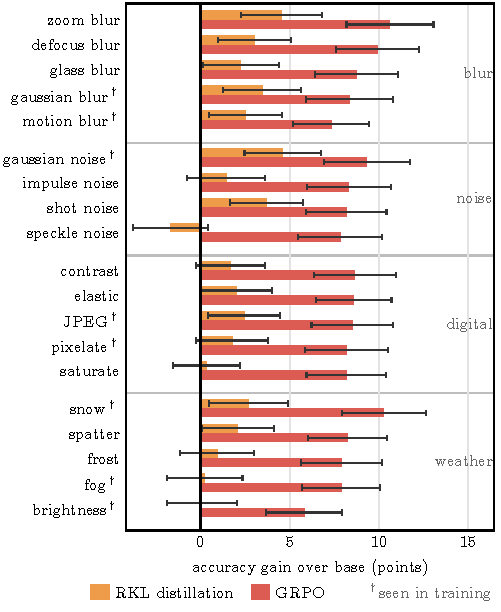
\includegraphics[width=\columnwidth]{figures/per_corruption_gain.pdf}
  \caption{Accuracy gain over the base Qwen3-VL-4B per corruption type (full fine-tuning), pooled over the
  corrupted TextVQA, GQA and VQAv2 questions of each type (all five severities, ${\sim}$1{,}190 questions each).
  Error bars: 95\% CI of the paired difference. $\dagger$: corruption type used in training.}
  \label{fig:per-corruption}
\end{figure}

\Cref{tab:accuracy} reports clean and corrupted accuracy. GRPO is strongest on every
dataset, raising corrupted GQA by $+10.2$ and corrupted VQAv2 by $+9.5$ over the base
model while also improving clean accuracy for Qwen3-VL-4B backbone; RKL improves the corrupted domain (\eg
$+4.2$ corrupted VQAv2) and holds clean accuracy flat. The gains are transfered to the corruption types that were not seen during the training \Cref{fig:per-corruption}. This means that improvements happen in a zero-shot manner and the gains for both the seen and unseen corruption types are similiar. The only regression that we can notice is for distillation which underperforms for speckle noise.  
% ---------------------------------------------------------------- Table 1 (main)
% ---------------------------------------------------------------- Table (main): accuracy
% ---------------------------------------------------------------- Table (main): accuracy
\begin{table}[t]
\centering
\caption{Accuracy (\%) on corrupted and clean images: unweighted mean over TextVQA, GQA and VQAv2
(full evaluation sets; per-benchmark numbers in Tab.~S1). A prediction is correct if the final answer
matches any annotator answer.}
\label{tab:accuracy}
\small
\setlength{\tabcolsep}{4pt}
\begin{tabular}{lcc}
\toprule
Method & Corrupted $\uparrow$ & Clean $\uparrow$ \\
\midrule
\multicolumn{3}{l}{\textit{Qwen3-VL-4B, full fine-tuning}} \\
Base                                         & 64.26 & 72.09 \\
RKL distillation                             & 66.39 & 72.16 \\
\quad + retraining, 10\% unanswerable        & 65.71 & 71.72 \\
\quad + steering, contrast, gated$^\dagger$  & 66.58 & 72.63 \\
\quad + steering, contrast, always$^\dagger$ & 65.59 & 71.69 \\
\quad + probe switch$^\dagger$               & 66.03 & 71.99 \\
GRPO                                         & 71.84 & 79.01 \\
\quad + retraining, 10\% unanswerable        & 71.61 & 78.48 \\
\quad + steering, no-image, gated$^\dagger$  & 71.96 & 79.01 \\
\quad + steering, no-image, always$^\dagger$ & 71.72 & 78.80 \\
\quad + probe switch$^\dagger$               & 68.16 & 76.46 \\
\midrule
\multicolumn{3}{l}{\textit{InternVL3.5-4B, full fine-tuning$^\ddagger$}} \\
Base                                         & 61.36 & 70.04 \\
RKL distillation (14B teacher)               & 66.66 & 74.06 \\
\quad + retraining, 10\% unanswerable        & 66.49 & 74.07 \\
\quad + steering, contrast, gated$^\dagger$  & 66.87 & 74.14 \\
\quad + steering, contrast, always$^\dagger$ & 66.57 & 74.16 \\
\quad + probe switch$^\dagger$               & 65.25 & 73.26 \\
GRPO                                         & 68.00 & 76.45 \\
\quad + retraining, 10\% unanswerable        & 67.58 & 75.83 \\
\quad + steering, no-image, gated$^\dagger$  & 68.03 & 76.46 \\
\quad + steering, no-image, always$^\dagger$ & 67.97 & 76.61 \\
\quad + probe switch$^\dagger$               & 66.73 & 75.79 \\
\midrule
\multicolumn{3}{l}{\textit{Gemma~3~4B, full fine-tuning$^\S$}} \\
Base                                         & 55.45 & 62.76 \\
RKL distillation (12B teacher)               & 58.94 & 65.79 \\
\quad + retraining, 10\% unanswerable        & 56.38 & 63.10 \\
GRPO                                         & 60.65 & 66.68 \\
\quad + retraining, 10\% unanswerable        & 60.71 & 67.66 \\
\quad + steering, contrast, gated$^\dagger$  & 60.40 & 66.81 \\
\quad + steering, contrast, always$^\dagger$ & 60.16 & 66.57 \\
\quad + steering, no-image, gated$^\dagger$  & 60.56 & 66.66 \\
\quad + steering, no-image, always$^\dagger$ & 60.70 & 66.90 \\
\quad + probe switch$^\dagger$               & 53.60 & 62.21 \\
\bottomrule
\end{tabular}
\end{table}


% ---------------------------------------------------------------- Table 2 (main)
% ---------------------------------------------------------------- Table (main): answering and refusal
% ---------------------------------------------------------------- Table (main): answering and refusal
% ---------------------------------------------------------------- Table (main): answering and refusal
% ---------------------------------------------------------------- Table (main): answering and refusal
\begin{table*}[t]
\centering
\caption{Answering and refusal (\%). Answerable accuracy and unnecessary refusals on the 2{,}934 answerable
VizWiz-val questions; correct refusals and accuracy on the 1{,}385 unanswerable ones; no-image refusals on
TextVQA, GQA and VQAv2 with the image withheld (mean of the three). A refusal is a final answer containing
``unanswerable'', ``cannot'', ``unable'', ``not possible'', ``impossible'', ``no image'', ``not visible'',
``not provided'' or ``not determin''. Accuracy counts an answer as correct if it matches any of the 10
annotator answers, so on unanswerable questions it also credits answers that some annotators gave.}
\label{tab:refusal}
\small
\begin{tabular}{lccccc}
\toprule
Method & Answerable acc.\ $\uparrow$ & Unnecessary refusals $\downarrow$ & Correct refusals $\uparrow$
       & Unanswerable acc.\ $\uparrow$ & No-image refusals $\uparrow$ \\
\midrule
\multicolumn{6}{l}{\textit{Qwen3-VL-4B, full fine-tuning}} \\
Base                                         & 51.0 & 12.8 & 71.6 & 76.0 & 52.0 \\
RKL distillation                             & 57.2 &  8.4 & 49.6 & 56.5 &  1.0 \\
\quad + retraining, 10\% unanswerable        & 58.6 & 13.3 & 61.7 & 66.9 &  2.2 \\
\quad + steering, contrast, gated$^\dagger$  & 59.1 & 11.1 & 57.5 & 64.1 &  1.6 \\
\quad + steering, contrast, always$^\dagger$ & 60.7 & 18.0 & 69.0 & 73.2 &  3.0 \\
\quad + probe switch$^\dagger$               & 63.1 & 20.1 & 87.5 & 90.4 & 54.1 \\
GRPO                                         & 63.5 &  3.2 & 44.9 & 60.3 &  0.5 \\
\quad + retraining, 10\% unanswerable        & 66.0 &  6.1 & 56.9 & 69.7 & 31.4 \\
\quad + steering, no-image, gated$^\dagger$  & 65.4 &  5.4 & 51.2 & 65.9 &  0.4 \\
\quad + steering, no-image, always$^\dagger$ & 68.7 & 14.5 & 70.7 & 81.7 &  0.4 \\
\quad + probe switch$^\dagger$               & 69.4 & 17.2 & 87.3 & 91.8 & 72.4 \\
\midrule
\multicolumn{6}{l}{\textit{InternVL3.5-4B, full fine-tuning$^\ddagger$}} \\
Base                                         & 50.7 & 11.2 & 58.6 & 64.5 &  2.0 \\
RKL distillation (14B teacher)               & 52.9 &  6.9 & 34.0 & 42.0 &  0.1 \\
\quad + retraining, 10\% unanswerable        & 57.7 & 14.6 & 62.7 & 67.2 &  2.0 \\
\quad + steering, contrast, gated$^\dagger$  & 52.4 &  7.2 & 35.2 & 42.9 &  0.1 \\
\quad + steering, contrast, always$^\dagger$ & 53.2 &  7.7 & 37.9 & 44.9 &  0.1 \\
\quad + probe switch$^\dagger$               & 60.0 & 23.1 & 87.4 & 89.1 & 49.5 \\
GRPO                                         & 55.7 &  2.5 & 25.9 & 39.0 &  0.0 \\
\quad + retraining, 10\% unanswerable        & 55.4 &  3.6 & 31.2 & 43.7 &  0.8 \\
\quad + steering, no-image, gated$^\dagger$  & 55.6 &  2.7 & 25.8 & 39.0 &  0.0 \\
\quad + steering, no-image, always$^\dagger$ & 55.4 &  3.2 & 29.5 & 41.4 &  0.1 \\
\quad + probe switch$^\dagger$               & 61.5 & 19.6 & 85.2 & 89.7 & 23.1 \\
\midrule
\multicolumn{6}{l}{\textit{Gemma~3~4B, full fine-tuning$^\S$}} \\
Base                                         & 51.6 &  5.0 & 28.2 & 34.4 &  2.1 \\
RKL distillation (12B teacher)               & 54.8 &  2.0 & 11.8 & 22.5 &  0.0 \\
\quad + retraining, 10\% unanswerable        & 55.1 &  4.2 & 25.8 & 35.0 &  1.4 \\
GRPO                                         & 49.2 &  0.4 & 10.9 & 24.5 &  0.0 \\
\quad + retraining, 10\% unanswerable        & 51.9 &  1.4 & 14.7 & 28.7 &  0.0 \\
\quad + steering, contrast, gated$^\dagger$  & 48.9 &  0.5 & 10.9 & 24.5 &  0.0 \\
\quad + steering, contrast, always$^\dagger$ & 48.6 &  0.5 & 10.0 & 23.9 &  0.0 \\
\quad + steering, no-image, gated$^\dagger$  & 49.1 &  0.6 & 12.1 & 26.1 &  0.0 \\
\quad + steering, no-image, always$^\dagger$ & 49.2 &  1.0 & 15.2 & 28.4 &  0.0 \\
\quad + probe switch$^\dagger$               & 57.4 & 17.9 & 80.6 & 85.6 & 99.8 \\
\bottomrule
\end{tabular}


\end{table*}









\paragraph{The silent abstention regression}
\label{sec:regression}

The same training degrades abstention. VizWiz-unanswerable accuracy (\cref{tab:refusal})
falls from $76.0$ (base) to $60.3$ (GRPO) and $56.5$ (RKL). The no-image test is sharper
(\cref{tab:refusal}): with the image withheld, base accuracy sits near the floor
($1.9$--$14.5$), but the fine-tuned models answer anyway, GRPO reaching $46.0$ on VQAv2
and $36.3$ on GQA. The most accurate model is the worst abstainer and nothing in the
accuracy columns of \cref{tab:accuracy} would reveal it.



\paragraph{Erased, or only suppressed?}
\label{sec:rq1}

A linear probe on frozen hidden states separates answerable from unanswerable VizWiz
questions at $\text{AUROC}\approx0.93$ in all three models, far above the shuffled-label
control (\cref{tab:probe}): fine-tuning does not erase the representation of
answerability. Among the unanswerable questions the models wrongly answered, the probe
still flags $76$--$77\%$ as unanswerable ($711$ items for RKL, $765$ for GRPO). The models
internally ``know'' these inputs are unanswerable, yet answer them. The lone exception is
image-missingness: with the image withheld (\cref{tab:probenoimg}) the flag rate
collapses for RKL (GQA $68\%\!\rightarrow\!31\%$), so distillation has partly lost its
sense that the image is gone, while GRPO keeps it. The failure is thus one of behavior,
not knowledge.

\begin{table}[tb]
\centering
\small
\caption{Answerability probe on frozen hidden states. Answerability is linearly decodable
at $\text{AUROC}\approx0.93$ after fine-tuning.}
\label{tab:probe}
\begin{tabular}{@{}lccc@{}}
\toprule
Model & Best layer & Probe AUROC & Shuffled \\
\midrule
Base               & 23 & 0.931 & 0.48 \\
Distillation (RKL) & 24 & 0.927 & 0.52 \\
GRPO               & 23 & 0.930 & 0.50 \\
\bottomrule
\end{tabular}
\end{table}

\begin{table}[tb]
\centering
\small
\caption{With the image withheld, share of questions the probe flags unanswerable. RKL
loses much of its sense that the image is missing.}
\label{tab:probenoimg}
\begin{tabular}{@{}lcccc@{}}
\toprule
Model & GQA & VQAv2 & TextVQA & VizWiz \\
\midrule
Base               & 68 & 75 & 98 & 100 \\
Distillation (RKL) & 31 & 38 & 94 & 99 \\
GRPO               & 56 & 64 & 98 & 100 \\
\bottomrule
\end{tabular}
\end{table}

\paragraph{Do the two recipes fail the same way?}
\label{sec:rq2}

They fail oppositely, and the reasoning-transplant test (\cref{tab:transplant}) shows it.
Handed a base ``can't-tell'' chain for a question it had answered, RKL abstains $98.4\%$
of the time: give it the right reasoning and it behaves correctly, so its own failure is
that it never produces that reasoning. Consistently, RKL's responses on these items are
far longer than the base model's or GRPO's: on the unanswerable set its median response
is $98$ tokens against $71$ (base) and $77$ (GRPO), and on the subset where it runs long
the gap widens to $341.5$ tokens against $\sim\!109$ for both others on the same questions
(\cref{tab:length})---the signature of an unsure, high-entropy chain that talks itself
into an answer, often running to the $768$-token limit. GRPO, given the identical chain,
still answers $91.8\%$ of the time: its reasoning is sound, but it has learned an
answer-level shortcut, committing to a definitive answer no matter what the chain
concludes, because exact-match reward always paid off for answering. In short, RKL cannot
reason its way to unanswerability; GRPO reasons there but will not act on it.

\begin{table}[tb]
\centering
\small
\caption{Reasoning transplant. Fraction that abstains when given a base ``can't-tell''
chain for a question it had answered. RKL fails on the reasoning side; GRPO on the answer
side.}
\label{tab:transplant}
\begin{tabular}{@{}lcc@{}}
\toprule
Model & Items & Refuses w/ ``can't-tell'' CoT \\
\midrule
Distillation (RKL) & 308 & 98.4\% \\
GRPO               & 389 & 8.2\% \\
\bottomrule
\end{tabular}
\end{table}



\paragraph{Recovering abstention without losing the gains}
\label{sec:rq3}

On every fine-tuned model, the probe switch restores abstention best. At a matched rate of
unnecessary refusals, the switch with $\tau{=}1$ recovers 73--77\% correct refusals on VizWiz
at 10--14\% unnecessary refusals. At a similar cost, retraining with the 10\% unanswerable mix
reaches 31--63\% and the best steering configuration 41--58\%. The switch also costs at most
1.2 points of corrupted accuracy, and it is the only remedy that consistently flags a missing
image (11--51\% of no-image questions, against at most 2\% for steering). The reason is that
robust fine-tuning suppresses abstention in the model's output but leaves answerability
linearly decodable from its residual stream. The switch reads this signal once, before
generation, and leaves the answer untouched when it does not fire, so the robustness gained on
answerable inputs is preserved, and a single threshold sets the trade-off ($\tau{=}0$ raises
correct refusals to 85--88\% at roughly twice the unnecessary refusals). Steering reads the
same representation but acts through one fixed direction added at every decoding step, so
triggering refusals and preserving answers conflict. On Qwen RKL, always-on no-image steering
reaches 88.6\% correct refusals but refuses 45.4\% of answerable questions and loses 8.9
points of accuracy. Steering is also fragile across models: the best direction differs between
models, and on Gemma~3 no configuration raises correct refusals by more than 7 points, whereas
the probe recipe, unchanged, lifts them from 11--13\% to 81--82\%. Retraining helps without
test-time machinery, but it needs a full training run and recovers less, because its
unanswerable examples are GQA questions on destroyed images, while real VizWiz questions are
unanswerable for subtler reasons (blur, framing, an object out of view). It also barely
teaches refusal on a missing image (0.8--2.2\%, except 31\% for Qwen GRPO). Distillation
absorbs the mix better than GRPO: the student is pulled toward a teacher that refuses readily
on destroyed images (RKL gains 13--29 points), whereas GRPO sees the label only through a
sparse exact-match reward (InternVL GRPO gains 5 points). Overall, abstention remains
recoverable after robust fine-tuning, and the cheapest remedy works best: one logistic
regression on 1{,}901 calibration questions, with no retraining and no change to decoding.




\section{Discussion and Conclusion}
\label{sec:conclusion}

A common way of training VLMs for corruption robustness quietly makes them worse at
admitting when they cannot see; standard accuracy benchmarks miss the regression; and it
is recoverable. The failure is behavioral, not representational (RQ1): answerability
stays linearly decodable after fine-tuning. The two dominant recipes fail for opposite
reasons (RQ2): distillation on the reasoning side, GRPO on the answer side via a
reward-induced shortcut. And the remedy should match the mechanism (RQ3): entropy-gated
steering for distillation, the missing unanswerable signal for GRPO---each at no cost to
corruption gains that already transfer zero-shot.

Our results also speak to a broader picture emerging from concurrent work. VLMs are now
understood to encode epistemic uncertainty internally while failing to express
it~\cite{pramono2026trapsbench,he2026knowing,chandu2025certainly}, a gap that probing and
steering expose in off-the-shelf models. We add the missing dynamic account: this gap is
not fixed, but is actively widened by a standard, well-motivated training objective, and
the widening is mechanistic enough that it can be diagnosed, attributed to the objective,
and reversed. That fine-tuning for one capability silently erodes another, in a direction
invisible to the metric being optimized, echoes what is seen when fine-tuning erodes
safety alignment~\cite{qi2024finetuning}, and is a pattern we expect to recur wherever a
training signal is defined only over answerable inputs.

The practical message is simple but consequential: wherever a confident wrong answer is
dangerous, corruption robustness and calibrated abstention must be measured, and
optimized, together.

\paragraph{Limitations.}
We study one backbone family and four benchmarks; whether the two failure signatures
generalize to other architectures, reward designs and corruption regimes is open.
Steering uses a single layer and a fixed gate threshold; adaptive, multi-layer and
per-token policies are natural extensions.

%%%%%%%%% REFERENCES
{
    \small
    \bibliographystyle{ieeenat_fullname}
    \bibliography{main}
}

\end{document}